\documentclass[12pt, a4paper]{book}\usepackage[]{graphicx}\usepackage[]{xcolor}
% maxwidth is the original width if it is less than linewidth
% otherwise use linewidth (to make sure the graphics do not exceed the margin)
\makeatletter
\def\maxwidth{ %
  \ifdim\Gin@nat@width>\linewidth
    \linewidth
  \else
    \Gin@nat@width
  \fi
}
\makeatother

\definecolor{fgcolor}{rgb}{0.345, 0.345, 0.345}
\newcommand{\hlnum}[1]{\textcolor[rgb]{0.686,0.059,0.569}{#1}}%
\newcommand{\hlsng}[1]{\textcolor[rgb]{0.192,0.494,0.8}{#1}}%
\newcommand{\hlcom}[1]{\textcolor[rgb]{0.678,0.584,0.686}{\textit{#1}}}%
\newcommand{\hlopt}[1]{\textcolor[rgb]{0,0,0}{#1}}%
\newcommand{\hldef}[1]{\textcolor[rgb]{0.345,0.345,0.345}{#1}}%
\newcommand{\hlkwa}[1]{\textcolor[rgb]{0.161,0.373,0.58}{\textbf{#1}}}%
\newcommand{\hlkwb}[1]{\textcolor[rgb]{0.69,0.353,0.396}{#1}}%
\newcommand{\hlkwc}[1]{\textcolor[rgb]{0.333,0.667,0.333}{#1}}%
\newcommand{\hlkwd}[1]{\textcolor[rgb]{0.737,0.353,0.396}{\textbf{#1}}}%
\let\hlipl\hlkwb

\usepackage{framed}
\makeatletter
\newenvironment{kframe}{%
 \def\at@end@of@kframe{}%
 \ifinner\ifhmode%
  \def\at@end@of@kframe{\end{minipage}}%
  \begin{minipage}{\columnwidth}%
 \fi\fi%
 \def\FrameCommand##1{\hskip\@totalleftmargin \hskip-\fboxsep
 \colorbox{shadecolor}{##1}\hskip-\fboxsep
     % There is no \\@totalrightmargin, so:
     \hskip-\linewidth \hskip-\@totalleftmargin \hskip\columnwidth}%
 \MakeFramed {\advance\hsize-\width
   \@totalleftmargin\z@ \linewidth\hsize
   \@setminipage}}%
 {\par\unskip\endMakeFramed%
 \at@end@of@kframe}
\makeatother

\definecolor{shadecolor}{rgb}{.97, .97, .97}
\definecolor{messagecolor}{rgb}{0, 0, 0}
\definecolor{warningcolor}{rgb}{1, 0, 1}
\definecolor{errorcolor}{rgb}{1, 0, 0}
\newenvironment{knitrout}{}{} % an empty environment to be redefined in TeX

\usepackage{alltt}
\usepackage{amsmath, float}

\title{Primer informe dinámico}
\author{Yajaira Toaquiza}
\date{\today}
\IfFileExists{upquote.sty}{\usepackage{upquote}}{}
\begin{document}

\maketitle

Este es el texto del primer informe automático generado por una Github Actions.\newline

Ahora vamos a probar el código generado para la ejecución automática del primer informe.

\begin{table}[H]
\centering
\begin{tabular}{|c|c|}\hline
\textbf{Provincia} & \textbf{Capital}\\ \hline
Pichincha & Quito\\ \hline
Guayas & Guayaquil\\ \hline
Azuay & Cuenca\\ \hline
\end{tabular}
\end{table}

Otro párrafo de prueba.



\begin{knitrout}
\definecolor{shadecolor}{rgb}{0.945, 0.992, 0.945}\color{fgcolor}\begin{kframe}
\begin{verbatim}
3 + 5 - 2
## [1] 6
rnorm(5, mean = 12, sd = 4)
## [1] 20.130109 12.288503 16.250226  3.590547 11.696390
\end{verbatim}
\end{kframe}
\end{knitrout}

A continuación nuestro segundo chunk
\begin{knitrout}
\definecolor{shadecolor}{rgb}{0.945, 0.992, 0.945}\color{fgcolor}
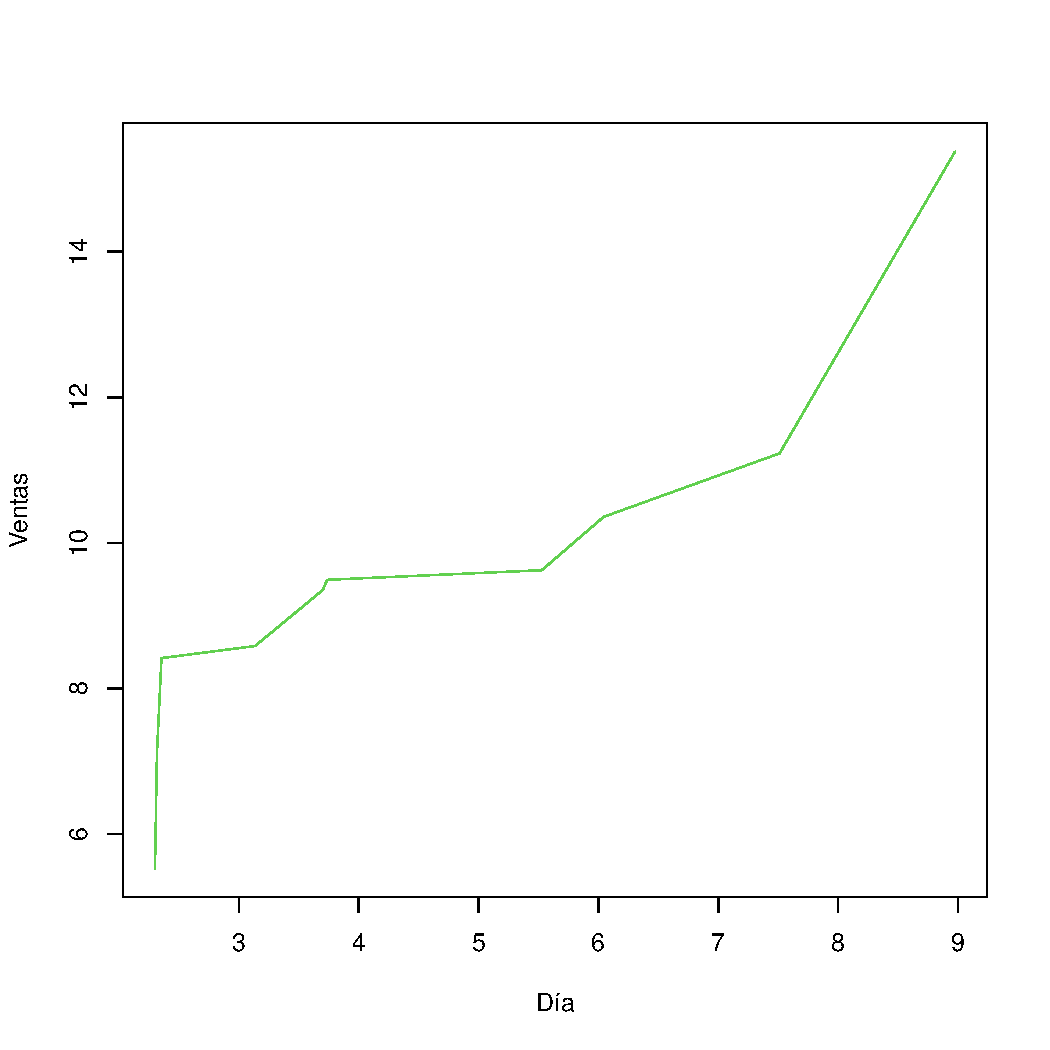
\includegraphics[width=\maxwidth]{figure/chunk02-1.pdf} 
\end{knitrout}




\end{document}
